% LuaLaTeX-ja を用いた卒業論文テンプレート（内容更新版）
\documentclass[a4paper,11pt]{ltjsreport}

%======================= パッケージ =======================
\usepackage{luatexja}
\usepackage{amsmath,amssymb}
\usepackage{bm}
\usepackage{graphicx}
\usepackage{ascmac}
\usepackage[top=20mm,bottom=30mm,left=20mm,right=20mm]{geometry}
\usepackage{multirow}
\usepackage{tabularx}
\usepackage{url}
\usepackage{color}
\usepackage{pgfplots}
\pgfplotsset{compat=1.18}
\newcolumntype{Y}{>{\raggedright\arraybackslash}X}
\usepgfplotslibrary{groupplots}
\renewcommand{\bibname}{参考文献}

%======================= 本文開始 =========================
\begin{document}

%--------------------- 表紙 ---------------------
\begin{titlepage}
  \centering
  ~~\vspace{1cm}
 
  {\Huge 卒　業　研　究　論　文 \par}
  {\Huge （2025年度）\par}

  \vspace{8cm}

  \begin{tabular}{rl}
    {\LARGE 題　　目}　 & {\LARGE ：低コスト移動ロボットによる} \\
                         & {\LARGE ~~VLM を用いた目標物体への自律移動} \\ \\ \\
    {\LARGE 指導教員}　 & {\LARGE ：保坂 忠明} \\　 \\ \\
    {\LARGE 学生番号}　 & {\LARGE ：1512221209} \\　 \\ \\
    {\LARGE 氏　　名}　 & {\LARGE ：小坂 尚璃}
  \end{tabular}

  \vfil
  \begin{flushright}
    明治大学理工学部 電気電子生命学科
  \end{flushright}
\end{titlepage}

\tableofcontents

%===========================================================
\chapter{序論}
\label{chap:intro}
\section{研究背景}
近年，画像と言語を同時に扱う基盤モデル（Vision-Language Model, VLM）が普及し，ロボットの行動決定に直接組み込む研究が活発化している。
その研究動向の中心にあるのは，(1) Web 画像やキャプションから学習した一般知識をもとに未知物体や抽象的な指示にも対処できるようにすること，および (2) 環境内の物体やランドマークをクラスラベルなどの意味情報とともに表現した地図を構築し，その上でナビゲーションを行うことである。
これらのアプローチでは，多様なセンサ情報と高い計算資源を前提とし，豊富な事前学習知識を活かした柔軟なナビゲーション性能が報告されている。
一方，教育・ホビー用途や簡易な現場計測のために用いられる低コスト移動ロボットでは，専用 GPU や高精度センサを搭載することは現実的でない。このような場面では，Raspberry Pi 等の小型コンピュータと単一カメラのみを搭載した機体から画像を取得し，外部 PC やクラウド上の VLM に推論をオフロードして進行方向を決定する構成が有力な選択肢となる。地図を作成・保持・参照せず，単一フレーム画像から直接「次の行動」を決めるため，セットアップが短時間で済み，環境変更時のリセット負荷も小さいという利点がある。
しかし，このような地図非依存・単眼カメラ依存の構成では，視覚ノイズや照度変化により判断が乱れやすく，VLM 推論に数秒以上を要する場合には遅延中に機体が進み過ぎる問題が生じる。高機能な VLM を用いても，この種の構成でどの程度安定した追従動作が得られるか，照度や初期位置ずれ，推論遅延が走行安定性にどのような影響を与えるかについては，体系的な実験報告が十分とはいえない。
低コスト移動ロボットにとっては，このシンプルな構成が現実的な選択肢であり，その性能限界と典型的な失敗パターンを実走行で把握することは，教育・プロトタイピングにおける VLM 活用の実装指針として重要である。

\section{先行研究と課題}
本節では，VLM を用いたロボット制御に関する先行研究を概観し，本研究との相違点と課題を整理する。

近年の代表的な研究として，RT-2\cite{rt2} および VL-Maps\cite{vlmaps} が挙げられる。RT-2 は，Web 上の画像およびテキストで事前学習したモデルをロボットデータで追加学習し，カメラ画像とテキスト指示を入力として，ロボットアームが「どの物体を，どの順番で，どのように動かすか」といった操作手順を直接出力する手法である。これにより，未知物体や多様な表現を含む指示に対しても，把持や配置といった操作をゼロショットで生成可能であることが示されている。ただし，GPU を搭載した計算機および高精度センサを備えたロボットプラットフォームを前提としている。

VL-Maps は，移動ロボットが走行中に取得したカメラ画像から，「どこに」「何が」存在するかという意味情報を環境地図上に逐次書き込むことで，意味ラベル付き地図を構築する手法である。利用者が「椅子の近く」「ソファとテレビのあいだ」などの文章で目的地を指定すると，この地図を検索して適切な位置を推定し，そこまでの経路を計画する。あらかじめ物体位置を教えなくても言語による柔軟な目的地指定が可能である一方，地図の構築と検索には高い計算能力とメモリ資源を要する。

これらのアプローチは，未知物体や新しい言い回しにも対応できる汎用性を有するが，いずれも GPU 搭載マシンや複数センサを備えた高価なロボットを前提としており，教育・ホビー用途の低価格ロボットにそのまま適用することは難しい。

これに対して本研究は，低価格の移動ロボットを対象とし，搭載計算資源やセンサ構成が大きく制約された環境を想定する。そのため，単眼カメラで撮影した画像を外部 PC 上の VLM に送信し，得られた出力から「前進」「左」「右」といった単純なコマンドを生成してロボットを制御する，地図非依存の簡潔な構成を採用する。

この構成には，部品コストや準備時間を抑えられるという利点がある一方で，いくつかの問題が想定される。第一に，VLM の推論に数秒を要する場合，その間もロボットは走行を続けるため，指令と実際の位置のずれが生じやすい。第二に，照明条件やカメラの揺れによって画像が変化すると，VLM の出力が不安定になり，ターゲット追従が破綻する可能性がある。第三に，初期位置がわずかに異なるだけでも，遅延や認識誤りが累積し，軌道の分岐を引き起こすことが考えられる。

高性能ロボットを前提とする先行研究では，これらの要因は主たる検討対象とはなってこなかった。しかし，低コスト移動ロボットで VLM を実用的に活用するためには，上記のような要因が走行安定性に与える影響を実機実験により定量的に把握することが重要である。本研究はこの点に着目し，単眼カメラと外部 VLM のみを用いた最小構成においてターゲット追従実験を行い，遅延・照度・初期位置ずれが走行結果に与える影響を明らかにすることを目的とする。

\begin{figure}[htbp]
  \centering
  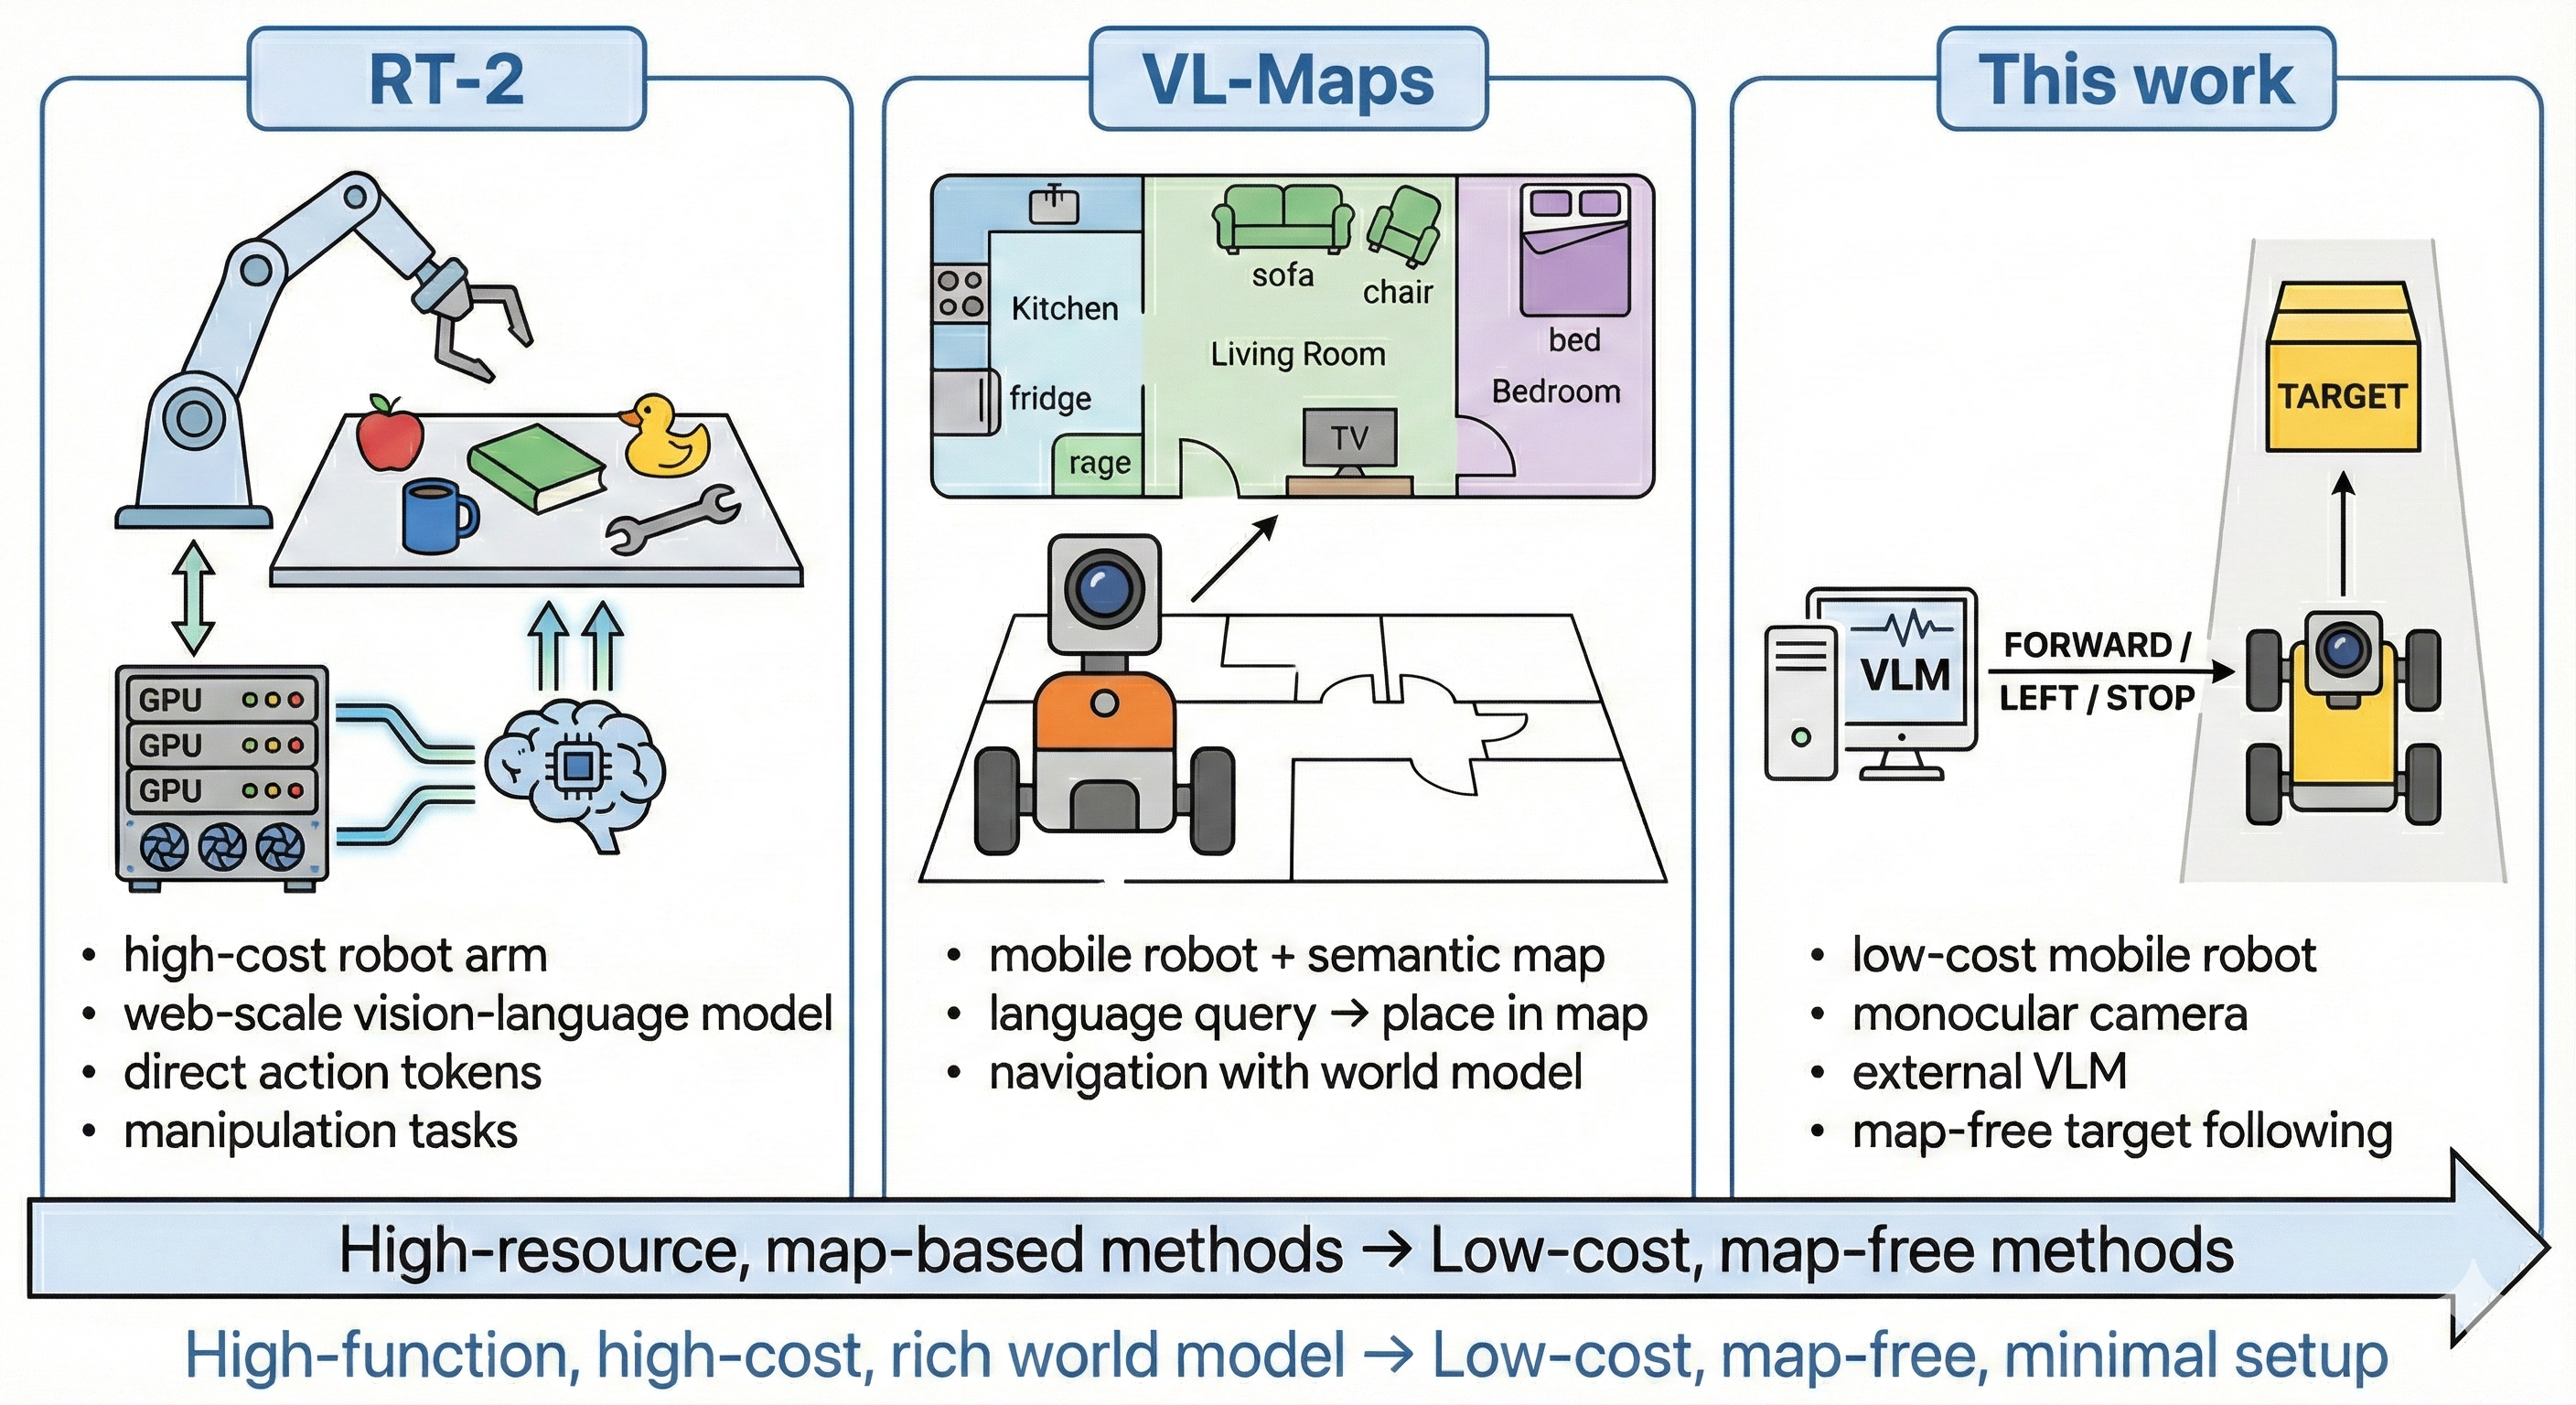
\includegraphics[width=\textwidth]{figs/fig1-1-positioning.png}
  \caption{RT-2・VL-Maps と本研究の位置づけの概念図}
  \label{fig:positioning}
\end{figure}

\section{研究目的}
本研究の目的は，教育・ホビー向けに現実的な「地図なし・単眼カメラ・外部 VLM」構成において，ターゲット追従がどの程度安定して動作しうるかを実走行で評価し，遅延・照度・初期位置ずれが成功率や到達時間，コマンド反転といった走行特性に与える影響を明らかにすることである。
具体的には，OSOYOO 社製 Raspberry Pi Robot Car で取得した画像を PC 側で推論し，視覚判断のみで「黄色いターゲットボックス（以下，ターゲット）に接近し，ターゲットが画像内で十分大きく写った時点で停止する」タスクを遂行させる。明るい環境（照度 873 lx）での走行試行を基準とし，低照度環境（照度 99.9 lx および 23.6 lx）および初期位置ずれ条件での試行を追加する。ログと取得画像から到達可否，所要時間，コマンド反転，推論遅延を取得し，教育・プロトタイピングで再現しやすい実験条件と結果の傾向として整理する。
実施範囲が限定されているため，網羅的な定量化には追加実験が必要であり，本稿では実施した条件における走行特性と，観察された範囲での失敗例について報告する。

\section{論文構成}
本論文の構成を示す。第\ref{chap:method}章でハードウェアと制御手順を述べる。第\ref{chap:experiments}章で実験環境と計測項目を説明し，第\ref{chap:results}章で結果を示す。第\ref{chap:discussion}章で考察を行い，第\ref{chap:conclusion}章で結論と今後の課題を述べる。

%===========================================================
\chapter{手法}
\label{chap:method}

\section{ハードウェア構成}
対象機体は OSOYOO社製 Raspberry Pi Robot Car（2023版）である。計算機として Raspberry Pi 5（8GB RAM）を搭載し，広角 USB カメラ，モータドライバ（L298N），ステアリング用サーボから構成する。カメラ解像度は 640×480，フレームレートは 5 fps とし，走行は室内の平坦な床面（長さ約 2.5 m の直線区間）で行う。実験機体の外観とカメラ搭載位置を図\ref{fig:robot}に示す。

\begin{figure}[htbp]
  \centering
  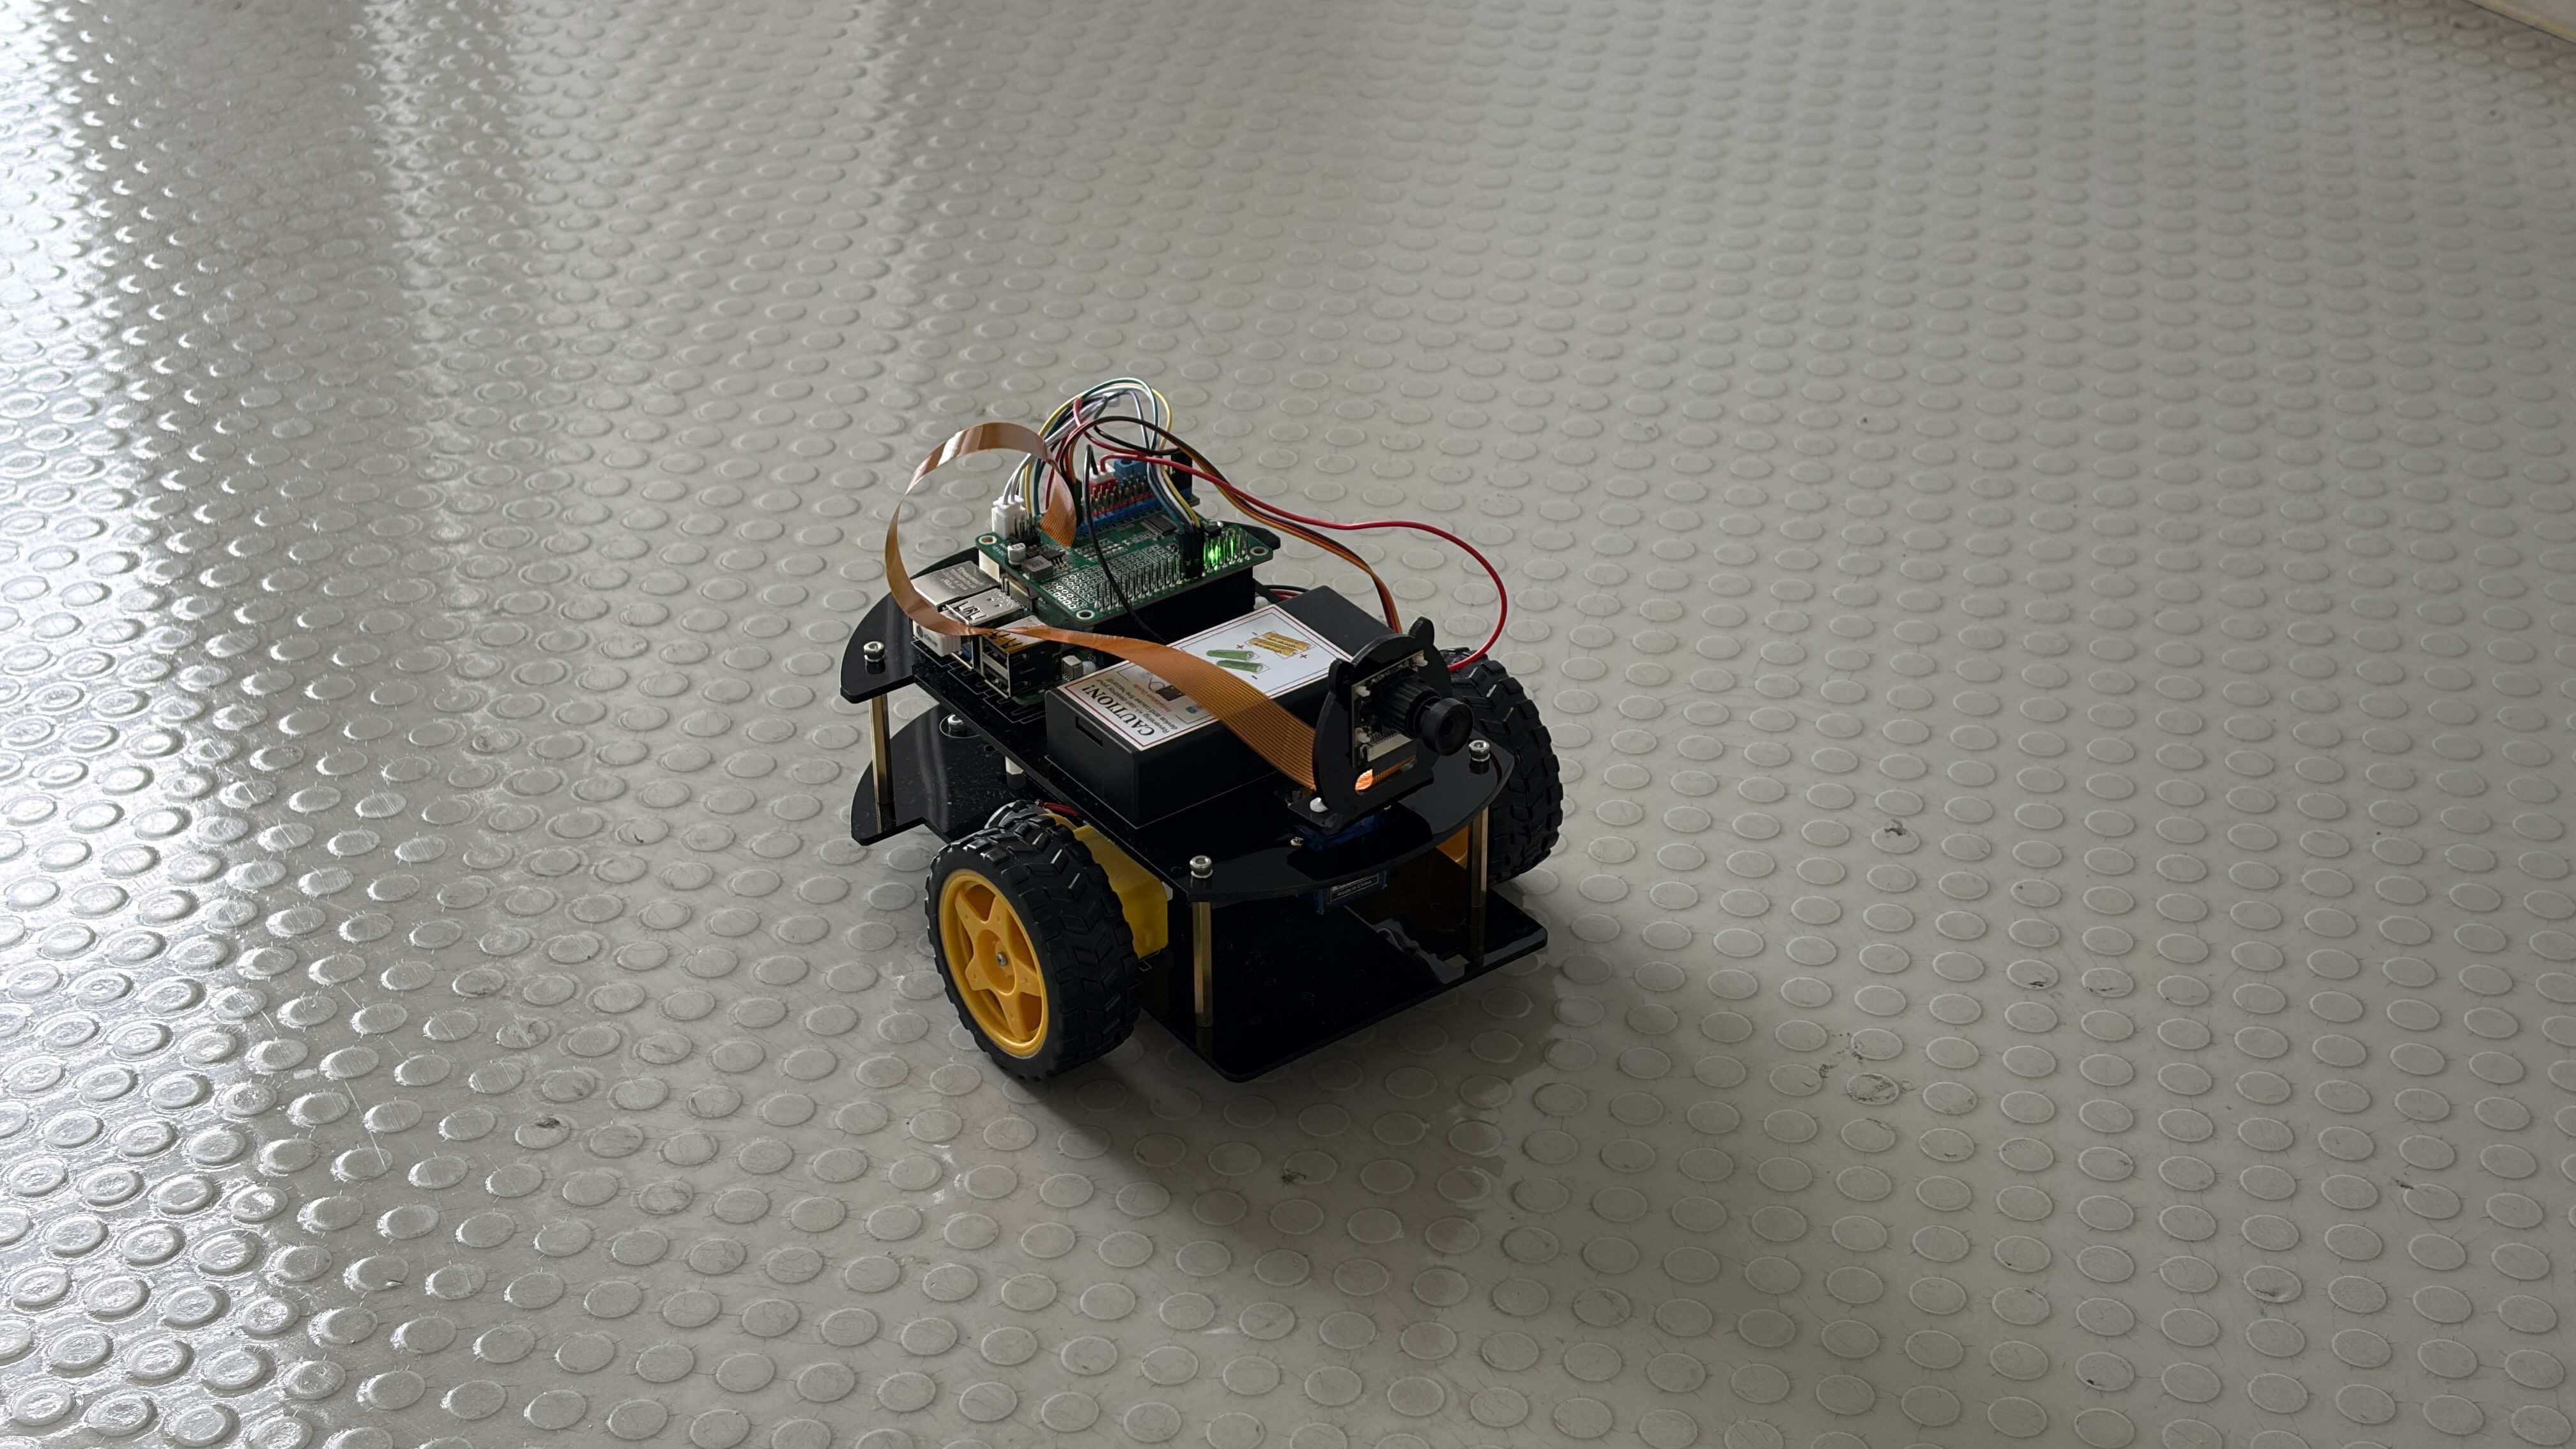
\includegraphics[width=0.9\textwidth]{figs/fig2-1-robot.jpg}
  \caption{実験機体（OSOYOO社製 Raspberry Pi Robot Car）とカメラ搭載位置}
  \label{fig:robot}
\end{figure}

\section{通信とソフトウェア構成}
本節では，図\ref{fig:system}に示すように，Raspberry Pi 側と PC 側で構成される通信・ソフトウェア構成の概要を述べる。Raspberry Pi 上では，カメラ画像の取得とモータ・ステアリング制御を行う HTTP サーバ \texttt{raspycar.raspi\_agent} を 8080 番ポートで起動した。サーバは，広角 USB カメラからの 640×480，5 fps の映像から最新フレームを取得し，\texttt{GET /frame.jpg} および \texttt{GET /stream.mjpg} で配信する。また，\texttt{POST /command} に対して \texttt{FORWARD}，\texttt{FORWARD\_SLOW}，\texttt{LEFT}，\texttt{RIGHT}，\texttt{BACK}，\texttt{STOP} のいずれかの文字列を受信すると，内部で左右モータへの速度指令に変換してモータドライバ L298N を駆動する。

PC 側からは同一ネットワーク上の Raspberry Pi に HTTP でアクセスし，\texttt{/frame.jpg} から一定間隔で 1 枚の画像を取得して VLM に入力する。VLM の応答として得られた一語のコマンド（\texttt{FORWARD}，\texttt{FORWARD\_SLOW}，\texttt{LEFT}，\texttt{RIGHT}，\texttt{BACK}，\texttt{STOP} のいずれか）をそのまま \texttt{/command} に送信し，ロボットを制御する。推論結果および送信時刻は PC 側でログとして保存し，後の解析に用いる。以上の一連の流れを概念的に示したものが図\ref{fig:system}である。

\begin{figure}[htbp]
  \centering
  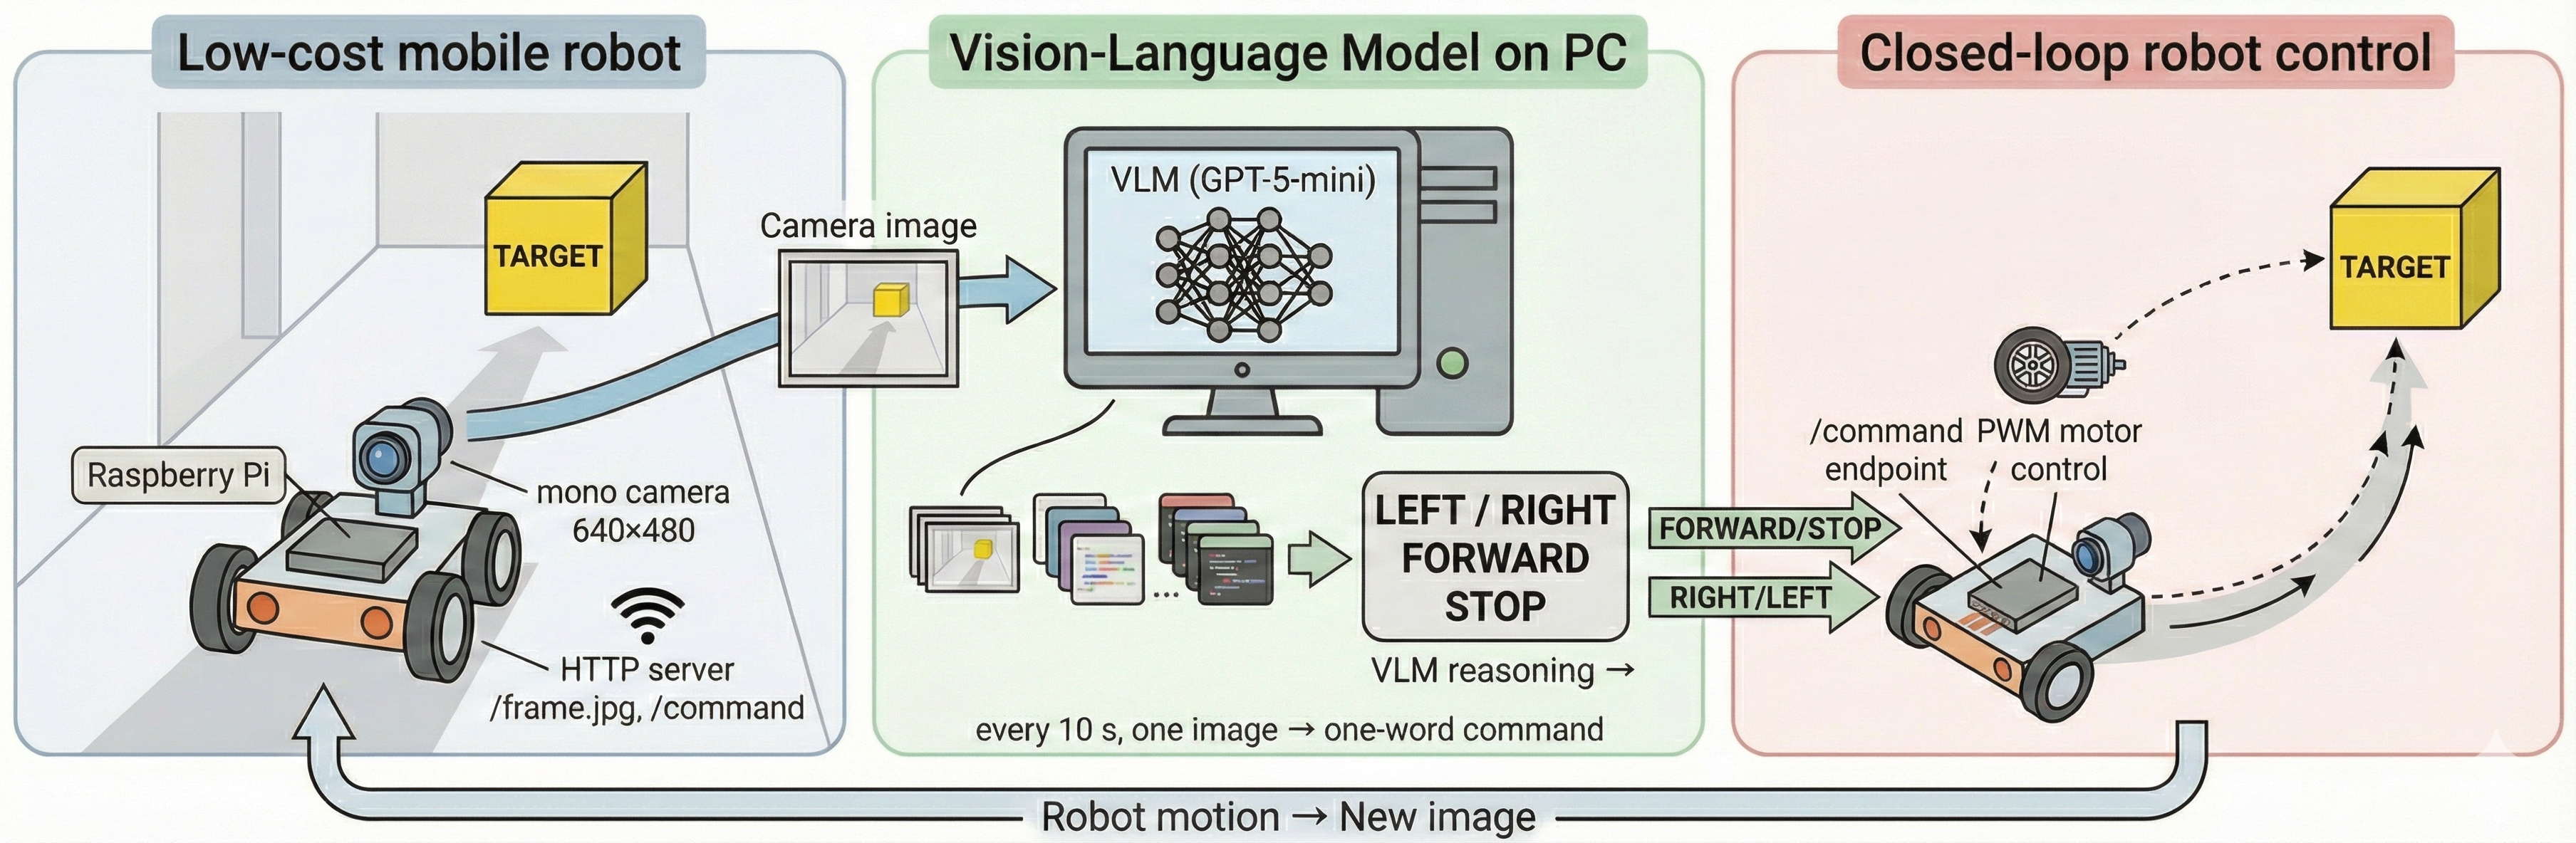
\includegraphics[width=\textwidth]{figs/fig2-2-system.png}
  \caption{提案構成：カメラ画像を外部 VLM で推論し，一語コマンドでロボットを制御するループ}
  \label{fig:system}
\end{figure}

\section{使用モデルとプロンプト}
機体から取得した画像を PC 側で推論する際に使用する VLM として GPT-5-mini-20250807（ローカル実行）を採用した。単一フレーム画像とテキストプロンプトを入力とし，VLM からは一語の行動コマンドを出力させる。
本研究では，(1) モデルの役割と出力形式を定義するシステムプロンプトと，(2) 各フレームと同時に送るデフォルトのタスク指示（\texttt{DEFAULT\_INSTRUCTION}）を区別して用いる。実装上は \texttt{pc\_controller\_direct\_gpt.py} 内で連続して定義し，推論時には両方を毎回送信している。以下にそれぞれの全文を示す。

\textbf{システムプロンプト（固定）}
\begin{quote}
You output only the next driving command as a single uppercase token from \{LEFT, RIGHT,\\ FORWARD, FORWARD\_SLOW, STOP\}. If a yellow box is visible, move toward it.\\ If no yellow box is visible, output STOP.
\end{quote}

\textbf{タスク指示（画像と同時に付与する \texttt{DEFAULT\_INSTRUCTION})}
\begin{quote}\footnotesize
\begin{verbatim}
DEFAULT_INSTRUCTION = (
    "Look at the image. Choose ONE from LEFT, RIGHT, FORWARD, FORWARD_SLOW, STOP. "
    "- If you see a yellow box (with or without the word TARGET): move toward it (LEFT/RIGHT to center it, 
    FORWARD/FORWARD_SLOW to approach). When it is very close or fills most of the frame, output STOP."
    "- If NO yellow box is visible at all: output STOP (do not advance blindly)."
)
\end{verbatim}
\end{quote}

上記プロンプトの動作を日本語で整理すると，次のようになる。
\begin{itemize}
  \item 応答は \texttt{LEFT}，\texttt{RIGHT}，\texttt{FORWARD}，\texttt{FORWARD\_SLOW}，\texttt{STOP} のいずれか一語に限定し，大文字で返す。
  \item フレーム内のどこかに黄色いボックス（「TARGET」の文字有無を問わない）が見えた場合は，即座に \texttt{STOP} を返す。
  \item 黄色いボックスが全く見えない場合は，探索を継続するため \texttt{FORWARD\_SLOW} を返す。
  \item 応答に説明や補足文を含めず，一語のみを出力する。
\end{itemize}

以降では，この \texttt{DEFAULT\_INSTRUCTION} を毎回画像とともに与える前提で，画像から直接次の行動を選択する VLM ベース制御として議論する。

\section{制御手順}
本研究では，画像取得からコマンド送信までの一連の処理を 10\,s ごとに繰り返す構成とした。各 10\,s の更新周期ごとに最新フレームを 1 枚取得して命令を更新する。

各更新では，(1) 直近フレームの取得，(2) VLM への送信と一語応答の取得，(3) 応答をモータ指令に変換して送信，(4) 応答と送信時刻のログ化，の順に実行する。
モータ指令は，「$-1$〜$1$ の範囲の数値で速さと向きを表し，その数値をモータへの電圧に変換する」という内訳で実装した。具体的には，正規化された値 $v \in [-1,1]$ を左右ホイールに与え，
\begin{itemize}
  \item $v$ が負のとき：前進方向
  \item $v$ が正のとき：後退方向
  \item $\lvert v\rvert$ の大きさ：モータ出力の強さ（速さ）
\end{itemize}
と解釈する。内部では $\lvert v\rvert$ をモータへの「オン時間の割合」（PWM デューティ比）に変換し，$v$ の符号に応じてモータドライバ L298N の方向ピンを切り替える。たとえば $v=-0.35$ は「前進方向で出力 35\% 程度」，$v=-0.14$ は「それより弱い前進」という意味になる。
本研究では，前進コマンド \texttt{FORWARD} に対して，左右ホイールの目標値をおおよそ $v=-0.35$ 付近に設定し，減速前進 \texttt{FORWARD\_SLOW} では \texttt{slow\_ratio}=0.4 を乗じた $v\simeq -0.14$ を用いた。左右旋回の \texttt{LEFT}，\texttt{RIGHT} では，左右ホイールの出力差を小さくつけることで，緩やかな弧を描くように旋回させている。具体的には，右旋回（\texttt{RIGHT}）のときは右ホイールを弱く，左ホイールを強く駆動し，左旋回（\texttt{LEFT}）のときはその逆とした。

\texttt{/command} という HTTP のエンドポイント（コマンドを受け付ける窓口）にコマンドを 1 回送信すると，その時点で左右モータの出力が更新される。この出力は，次のコマンドが届くか，一定時間コマンドが届かずに安全装置（ウォッチドッグ）が作動して \texttt{STOP} に切り替わるまで保持される。そのため，1 回のコマンドで実際に何秒間動くかは，更新周期（本研究では 10\,s）とウォッチドッグのタイムアウト設定に依存する。
安全のため，VLM から連続して \texttt{STOP} が返った場合はモータを無通電とし，外部操作によってのみ走行を再開できるようにした。

\section{走行特性の簡易測定}
本節では，本実験に先立って実施した簡易な走行特性の測定結果について述べる。低コスト機体では，モータの個体差やタイヤのネジの締まり具合，床面の摩擦，バッテリ電圧の違いにより，同じ指令を与えても走行量が日ごとに変動しやすい。本研究でも，組み立て誤差を補正するためにステアリングサーボの中立角を \(-68^\circ\) に設定したうえで，左右モータの旋回癖を抑える目的で速度指令に対して \texttt{steer\_offset = 0.01} のオフセット補正を加えたところ，大まかには直進するものの，わずかに左右どちらかへ寄る挙動が残った。

そこで，ロボットを静止状態から単一のモータコマンドを 1 回だけ送信し，その後は追加コマンドを送らずに停止するまで走らせたときの変位を簡易に計測した。座標系は，走行開始時点の機体左上の角を原点とし，機体の横方向を $x$ 軸（右向きを正），縦方向を $y$ 軸（前方を正）とした。この座標系における代表的な変位を表\ref{tab:single_cmd}に示す。

これらの値は，当日の電圧と床面条件における一回計測に基づく近似値であり，指令と変位量の厳密な対応をモデル化したものではない。そのため，本研究では簡易測定の結果をあくまで参考情報として扱い，第\ref{chap:results}章で推論遅延と移動距離の関係を議論する際の目安として用いる。

\begin{table}[htbp]
  \centering
  \caption{単一コマンドによる変位（機体左上角を原点とした座標系）}
  \label{tab:single_cmd}
  \begin{tabular}{|c|c|c|c|}
    \hline
    指令 & $\Delta x$ [cm] & $\Delta y$ [cm] & 備考 \\
    \hline
    \texttt{FORWARD} & +1.0 & +31.7 & わずかに右寄りの前進 \\
    \texttt{RIGHT}   & +7.0 & +25.6 & 右方向へのアーク旋回 \\
    \texttt{LEFT}    & $-3.7$ & +27.4 & 左方向へのアーク旋回 \\
    \texttt{BACK}    & +5.2 & $-81.8$ & 後方への後退（前進より距離が大きい） \\
    \hline
  \end{tabular}
\end{table}

%===========================================================
\chapter{実験}
\label{chap:experiments}

\section{環境と照度}
本研究では，表\ref{tab:runs}に示す複数の試行条件のもとで，直線コース上のターゲット追従実験を行った。実験環境とターゲット配置の概観を図\ref{fig:course}に示す。長さ約 2.5 m の室内直線コースで床は平坦なフロア材とし，壁や背景は固定とした。ターゲットは終点に置いた黄色いボックス（“TARGET” と印字）である。
カメラ画像上の初期視野は，ターゲットが画面中央から水平 $\pm 10\%$，垂直方向は中央よりやや上，サイズは画面比 5--15\% となるように位置決めした。図\ref{fig:illum_samples}に，各照度条件におけるカメラ画像の例を示す。
ターゲット位置の基準を中央配置（初期視野で水平 $\pm 10\%$ 程度）に置き，これを右へ 68.8 cm，左へ 53.0 cm ずらした配置でも試行した。初期視野の水平方向ずれはおおよそ $\pm 20$--$25\%$ となる。

照度はターゲット設置位置に照度計を置いて測定し，明るい条件では 873 lx を維持した。比較のために，99.9 lx および 23.6 lx となるよう照明を落とした低照度条件を二水準用意した。本稿では，これら三水準をそれぞれ 873 lx，99.9 lx，23.6 lx と表記する。

\begin{figure}[htbp]
  \centering
  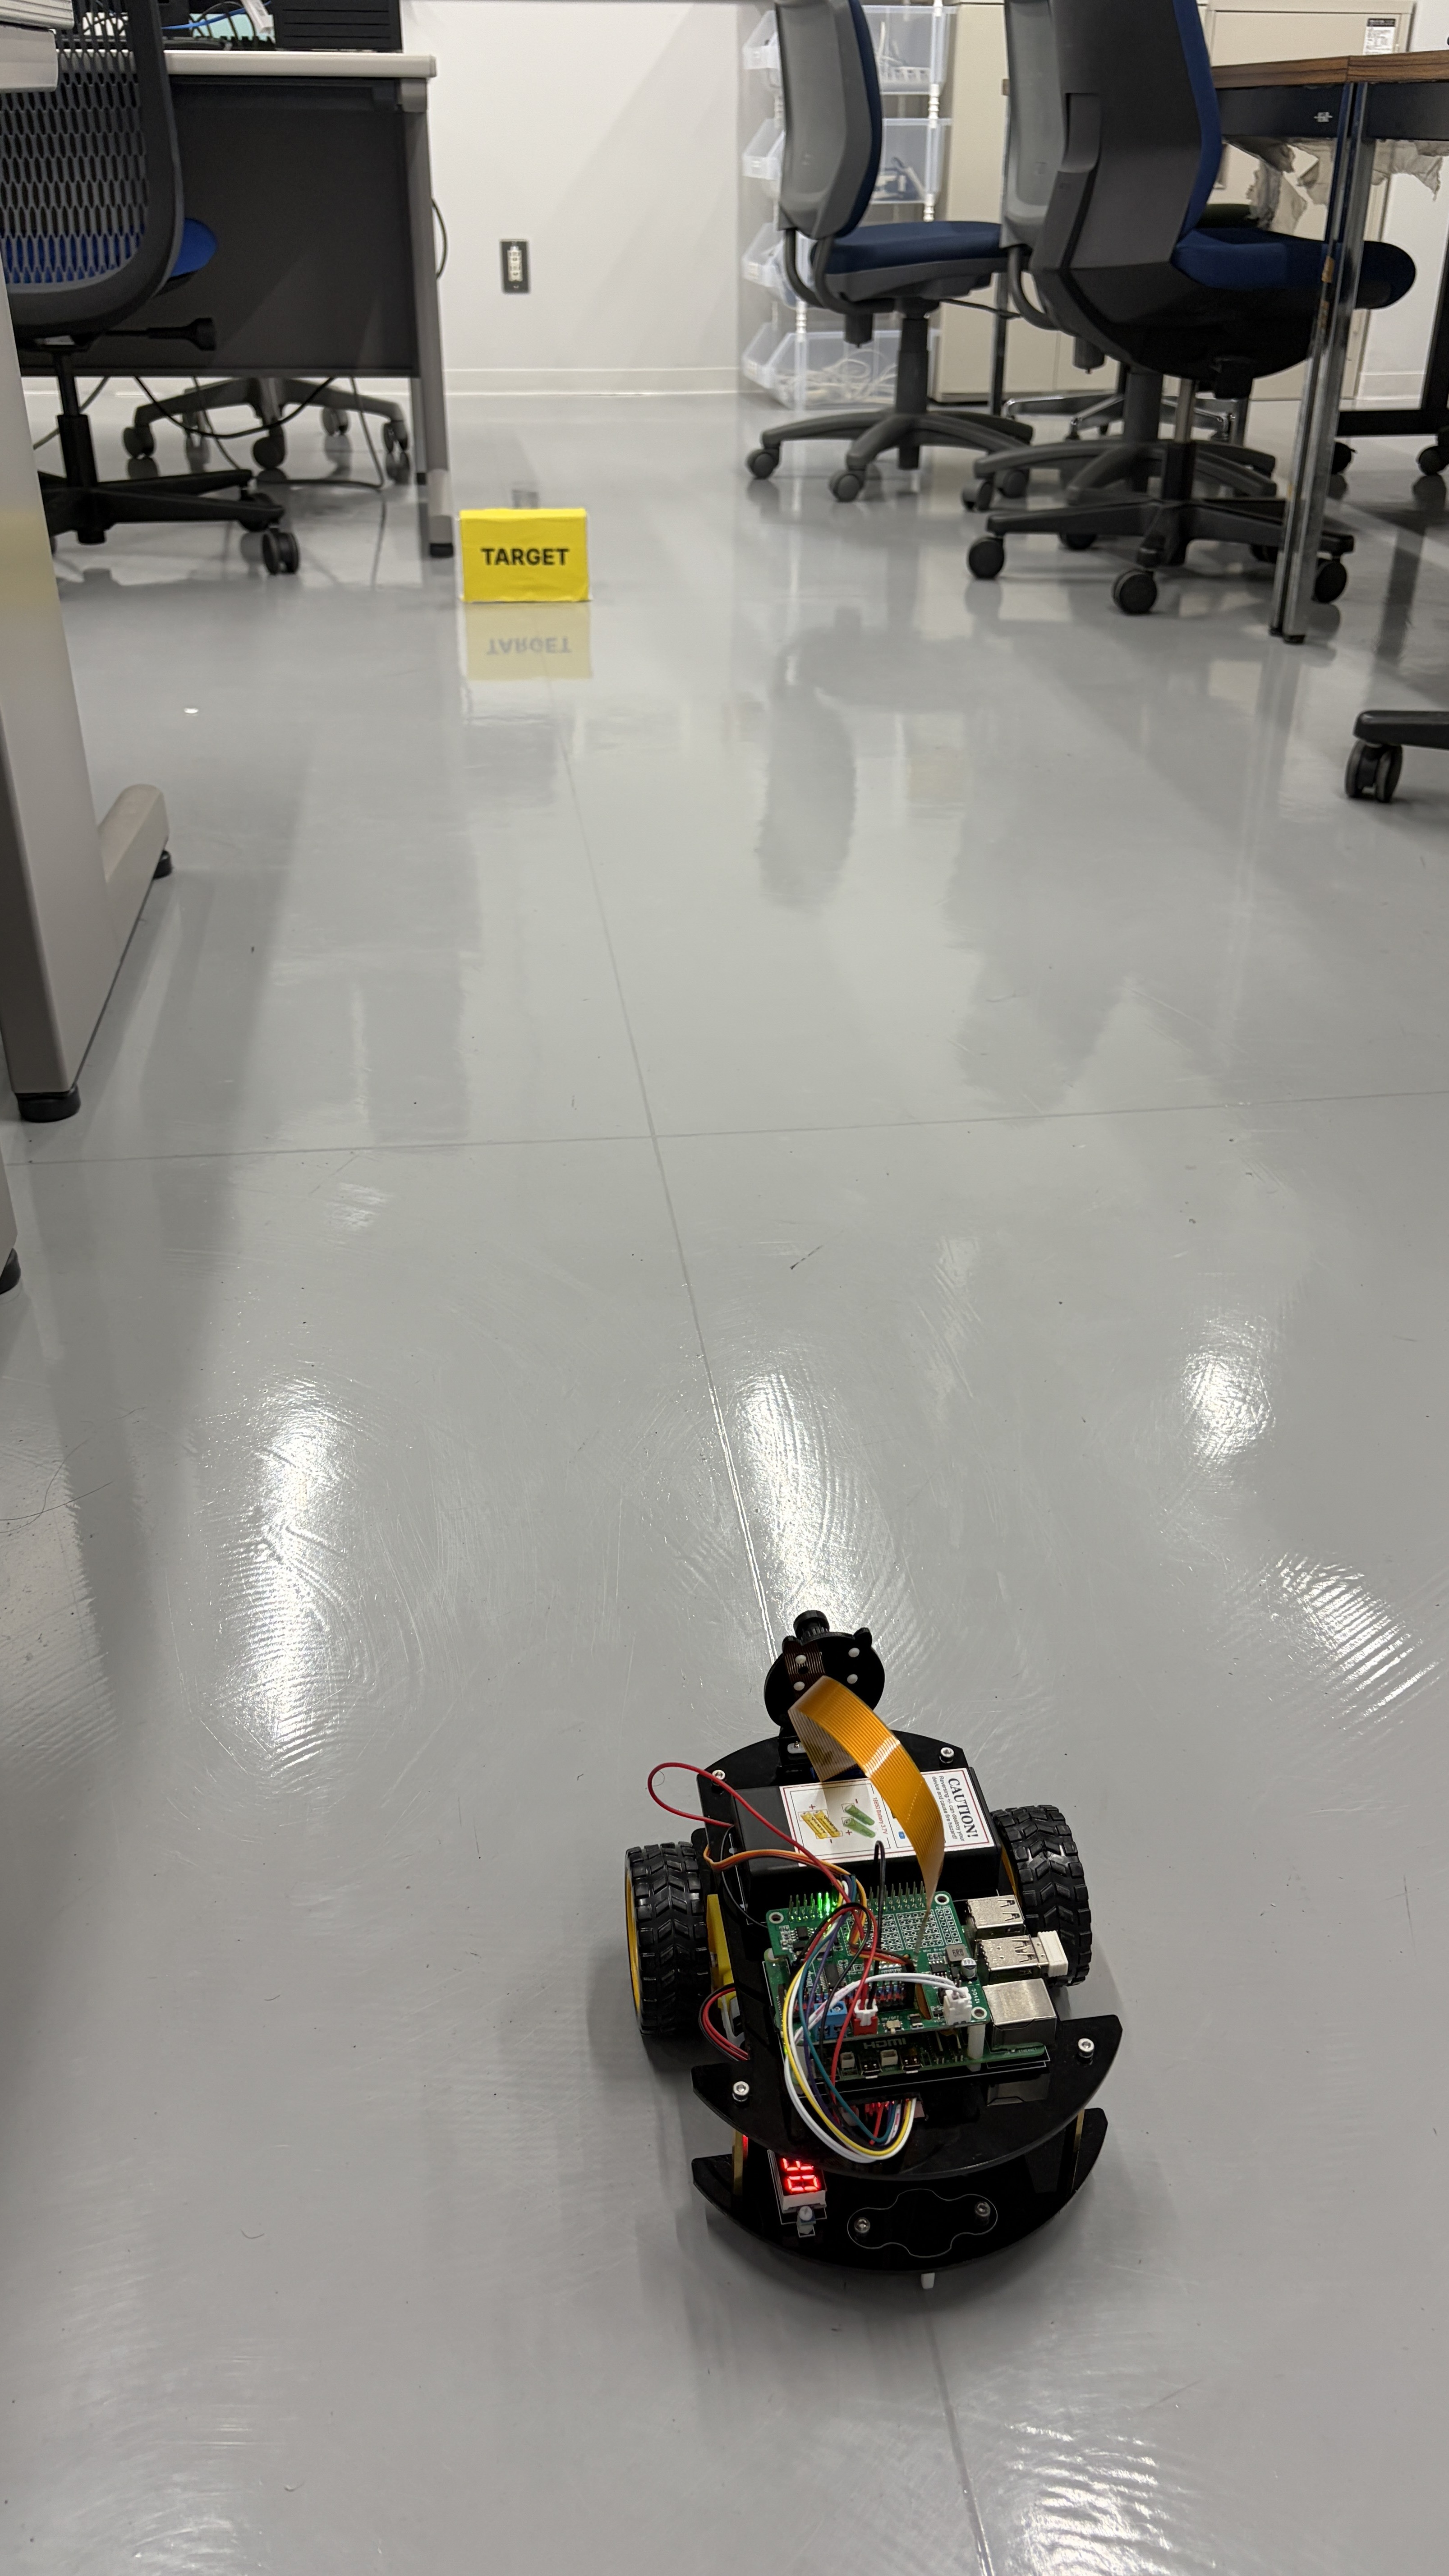
\includegraphics[width=0.58\textwidth]{figs/fig3-1-course.jpg}
  \caption{室内コースとターゲット配置（長さ約 2.5 m，照度はターゲット位置で測定）}
  \label{fig:course}
\end{figure}

\begin{figure}[htbp]
  \centering
  \begin{minipage}[t]{0.32\textwidth}
    \centering
    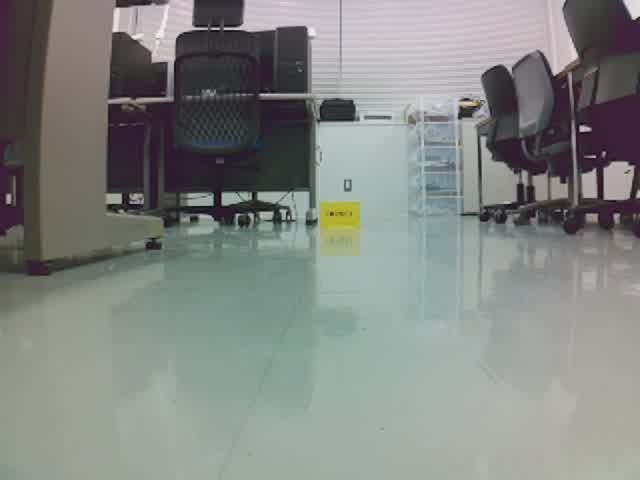
\includegraphics[width=\linewidth]{figs/fig3-2-873lx.jpg}\\[-2mm]
    {\small 873\,lx（明条件・中央配置）}
  \end{minipage}
  \hfill
  \begin{minipage}[t]{0.32\textwidth}
    \centering
    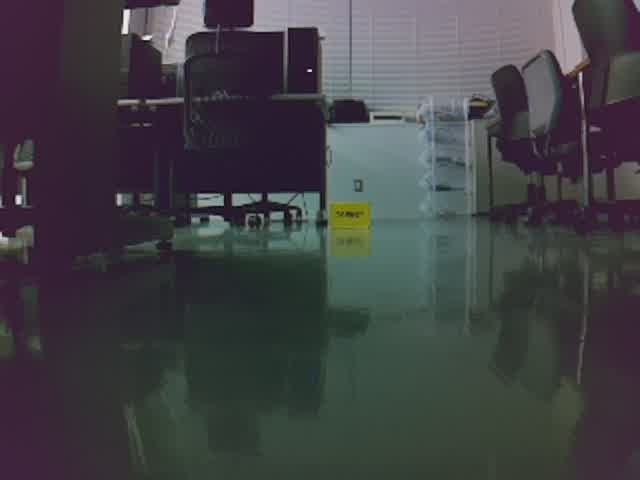
\includegraphics[width=\linewidth]{figs/fig3-2-99lx.jpg}\\[-2mm]
    {\small 99.9\,lx（低照度・中央配置）}
  \end{minipage}
  \hfill
  \begin{minipage}[t]{0.32\textwidth}
    \centering
    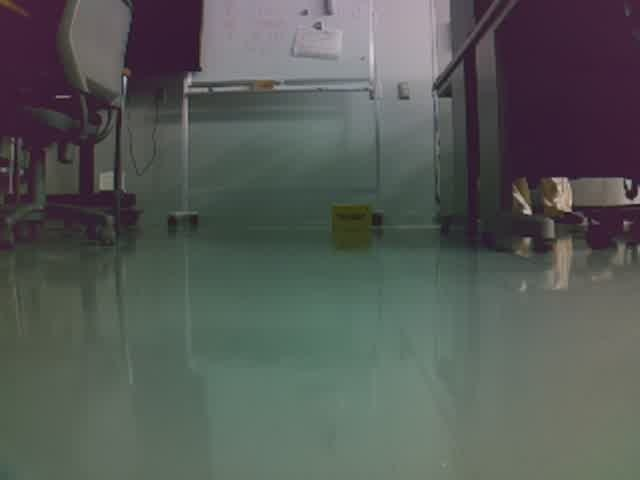
\includegraphics[width=\linewidth]{figs/fig3-2-23lx.jpg}\\[-2mm]
    {\small 23.6\,lx}
  \end{minipage}
  \caption{照度条件別のカメラ画像例（左：873\,lx 明条件・中央配置，中央：99.9\,lx 低照度・中央配置，右：23.6\,lx 低照度）。照度はターゲット位置で測定した。}
  \label{fig:illum_samples}
\end{figure}

\section{試行条件}
実施した試行条件の一覧を表\ref{tab:runs}に示す。本論文では，明条件（873 lx）・中央配置の条件を「試行A」，低照度 99.9 lx を「試行B」，低照度 23.6 lx を「試行C」，明条件でターゲットを基準位置から左右に移動した試行を「試行D1（右方向へ移動）」「試行D2（左方向へ移動）」と呼ぶ。
試行Aでは，明条件（873 lx）でターゲットが画面中央付近に写る状態から開始し，成功率や到達時間，コマンド反転回数，推論遅延を測定した。試行B, C では，照度のみをそれぞれ 99.9 lx および 23.6 lx に下げ，暗所での追従性能を確認した。試行D1, D2 では，3.1節で述べたようにターゲット位置を中央基準から左右へ移動させ，初期視野が水平方向にずれた状態での耐性を確認した。

各試行では，フレーム画像，VLM 応答，送信コマンド，タイムスタンプ，別カメラで取得した俯瞰画像を保存し，通し番号と照度，開始・終了時刻をメタデータとして付与した。VLM が \texttt{STOP} を 2 回連続で出力し，その時点で機体が静止している場合を「到達」とみなし，その時点で試行を終了した。

\begin{table}[htbp]
  \centering
  \caption{試行条件の構成}
  \label{tab:runs}
  \footnotesize
  \setlength{\tabcolsep}{3pt}
  \setlength{\arrayrulewidth}{0.5pt}
  \renewcommand{\arraystretch}{1.1}
  \begin{tabularx}{\textwidth}{|c|c|c|c|Y|}
    \hline
    試行 & 繰り返し回数 & 照度 [lx] & ターゲット位置 & 初期視野の条件 \\
    \hline
    試行A & 6回   & 873   & 中央 & 水平$\pm 10\%$，垂直は中央よりやや上，サイズ5--15\% \\
    試行B & 2回   & 99.9  & 中央 & 試行Aと同一 \\
    試行C & 2回   & 23.6  & 中央 & 試行Aと同一 \\
    試行D1 & 1回   & 873   & 右に 68.8 cm ずれ & 水平ずれ +20〜25\% \\
    試行D2 & 1回   & 873   & 左に 53.0 cm ずれ & 水平ずれ −20〜25\% \\
    \hline
  \end{tabularx}
  \vspace{1mm}
  \begin{flushleft}
    \footnotesize
    注：試行Aは基本条件として成功率・到達時間・反転回数・推論遅延を取得。試行B, C は照度のみ低下。試行D1, D2 はターゲットを基準位置から左右へ移動した配置。
  \end{flushleft}
\end{table}

\section{計測項目}
本稿で報告する主な指標は以下のとおりである。
\begin{itemize}
  \item 成功率：各試行条件ごとに実施した試行のうち，ターゲットが画像内で十分大きく写り，VLM が \texttt{STOP} を連続して出力し，その時点で機体が静止していたものの割合とする。

  \item 到達時間：1 回の試行の開始から，VLM が初めて \texttt{STOP} を出力したコマンドを送信するまでに要した時間とする。具体的には，「最初のコマンドを送信した時刻」から「\texttt{STOP} が初めて選ばれたコマンドを送信した時刻」までの差分を到達時間と定義する。到達時間は成功試行についてのみ定義し，失敗試行については「到達時間なし」として扱う。

  \item コマンド反転回数：連続する 2 回の指令が前後（\texttt{FORWARD} 系と \texttt{BACK}）または左右（\texttt{LEFT} と \texttt{RIGHT}）で正反対の内容になっているペアの数を数える。短い時間スケールで進行方向の指令が行ったり来たりすると，ロボットの動きがガタガタと不安定になる。この不安定さを定量的に把握することがコマンド反転回数の狙いである。

  \item 推論遅延：各コマンドについて，画像を VLM に送信してから一語の応答が返ってくるまでに要した時間とする。
\end{itemize}
これらの値は各試行ごとにログから取得し，第\ref{chap:results}章で試行単位の一覧として示す。

%===========================================================
\chapter{結果}
\label{chap:results}
\section{集計結果}
各試行ログから到達可否，VLM 推論結果，送信コマンド列，推論遅延を抽出し，3.3節で定義した指標を条件ごとに集計した結果を表\ref{tab:summary}に示す。各条件の試行回数は 2〜6 回と少ないため，本章では統計的有意差は主張せず，少数試行に基づく傾向として結果を解釈する。

\begin{table}[htbp]
  \centering
  \caption{各試行ログの計測値一覧（到達時間は最初のコマンド送信から最初の \texttt{STOP} まで）}
  \label{tab:summary}
  \footnotesize
  \setlength{\tabcolsep}{2.5pt}
  \setlength{\arrayrulewidth}{0.5pt}
  \renewcommand{\arraystretch}{1.1}
  \noindent\begin{tabularx}{\linewidth}{|c|c|l|X|c|c|c|}
    \hline
    試行 & 照度 [lx] & ログID & 成否・備考 & 到達時間 [s] & 反転回数 & 推論遅延[平均/最大] \\
    \hline
    試行A & 873 & 172549 & 失敗（通過） & --- & 1 & 1.41 / 2.71 \\
    試行A & 873 & 172908 & 成功 & 100.54 & 0 & 1.15 / 1.57 \\
    試行A & 873 & 173222 & 成功 & 100.32 & 0 & 1.10 / 1.55 \\
    試行A & 873 & 173500 & 成功 & 101.17 & 0 & 1.14 / 1.63 \\
    試行A & 873 & 173727 & 失敗（見失い） & ---  & 0 & 1.32 / 1.79 \\
    試行A & 873 & 173846 & 成功 & 90.48  & 0 & 1.08 / 1.65 \\
    \hline
    試行B & 99.9 & 174717 & 成功 & 112.98 & 0 & 1.21 / 1.90 \\
    試行B & 99.9 & 174444 & 失敗（通過） & --- & --- & --- \\
    \hline
    試行C & 23.6 & 175317 & 成功 & 124.19 & 2 & 1.24 / 2.54 \\
    試行C & 23.6 & 175030 & 失敗（通過） & --- & --- & --- \\
    \hline
    試行D1 & 873 & 175653 & 失敗（ターゲット右移動，手動停止） & --- & --- & --- \\
    \hline
    試行D2 & 873 & 180040 & 成功 & 123.63 & 0 & 1.14 / 1.88 \\
    \hline
  \end{tabularx}
\end{table}

明条件・中央視野の試行A（873 lx）は 6回中 4回が到達し，成功率は 66.7\% であった。到達した 4回の到達時間は 90--101\,s の範囲で，コマンド反転回数は最大 1 回，推論遅延は平均 1.21\,s，最大 2.71\,s で，多くのコマンドが 2\,s 未満で応答している。失敗した 172549 では \texttt{STOP} 直前に余分な \texttt{FORWARD} が選ばれてターゲットを通過し，173727 では途中でターゲットを見失ってコースアウトした。試行A における推定軌跡を図\ref{fig:trajectory1}に示す。成功試行ではほぼ直線的に TARGET 方向へ進む一方，失敗試行では途中で軌跡が途切れている。

低照度条件の試行B（99.9 lx）と試行C（23.6 lx）はそれぞれ 2回ずつ実施し，いずれも 1回のみ到達した（成功率 50.0\%）。成功試行の到達時間は試行Bで 113\,s，試行Cで 124\,s であり，明条件より 10--30\,s 程度長い。特に試行Cでは，図\ref{fig:illum_samples}右に示すようにカメラ画像上でターゲットのコントラストが低く，床面の反射に埋もれて見えにくい状態となっていた。このため，\texttt{LEFT}/\texttt{RIGHT} が行き来する反転が 2 回観測され，暗所ほど前後・左右の揺れが生じやすい傾向が示唆される。一方，推論遅延自体は明条件とほぼ同じ平均 1.2\,s であり，照度による大きな差は見られなかった。失敗側はいずれもターゲットを通過してしまうパターンであった。

ターゲットを基準位置から右へ 68.8\,cm 移動した試行D1（ログID 175653）が 1回失敗し，左へ 53.0\,cm 移動した試行D2が 1回成功した。試行D2の到達時間は 124\,s，反転回数は 0 回で，推論遅延は平均 1.14\,s，最大 1.88\,s であった。照度は試行Aと同程度であるにもかかわらず，初期視野の水平ずれにより到達に時間がかかり，少なくともターゲットを右へ移動した場合には失敗が生じた点は留意すべきである。

図\ref{fig:trajectory2}に，試行A における代表的な 1 試行のコマンド系列と推論遅延の時間推移を示す。上段の階段状プロットは，各時刻で出力されたコマンドが \texttt{FORWARD}，\texttt{LEFT}，\texttt{RIGHT}，\texttt{STOP} のどれであったかを表し，下段は各更新ごとの推論遅延である。推論遅延はすべて 2 s 未満である。一方で停止コマンドが出力されたのは 100\,s 付近の 2 回であり，その時点ではすでにターゲットを通過していたため，停止判断の遅れが失敗の主因となっている。

\begin{figure}[htbp]
  \centering
  \begin{tikzpicture}
    \begin{axis}[
      width=0.9\textwidth,
      height=7cm,
      grid=both,
      xmin=0,xmax=30,
      ymin=-20,ymax=290,
      xlabel={$x$ [cm] （右正）},
      ylabel={$y$ [cm] （前方正）},
      legend style={
        font=\scriptsize,
        at={(0.98,0.02)},
        anchor=south east,
        legend columns=3,
        legend cell align=left,
        fill=white,
        draw=none
      },
    ]
      % 成功トライアル（実験セット1, 873 lx）
      \addplot+[color=green!60!black, thick, mark=none] coordinates {
        (0,0)(1.0,31.7)(2.0,63.4)(9.0,89.0)(10.0,120.7)(11.0,152.4)(18.0,178.0)(19.0,209.7)(20.0,241.4)(27.0,267.0)
      }; \addlegendentry{172908（成功）};
      \addplot+[color=red, thick, mark=none] coordinates {
        (0,0)(1.0,31.7)(2.0,63.4)(9.0,89.0)(10.0,120.7)(11.0,152.4)(18.0,178.0)(19.0,209.7)(15.3,237.1)(11.6,264.5)
      }; \addlegendentry{173222（成功）};
      \addplot+[color=violet, thick, mark=none] coordinates {
        (0,0)(1.0,31.7)(2.0,63.4)(9.0,89.0)(10.0,120.7)(11.0,152.4)(18.0,178.0)(19.0,209.7)(20.0,241.4)(16.3,268.8)
      }; \addlegendentry{173500（成功）};
      \addplot+[color=brown!70!black, thick, mark=none] coordinates {
        (0,0)(1.0,31.7)(2.0,63.4)(9.0,89.0)(10.0,120.7)(11.0,152.4)(12.0,184.1)(19.0,209.7)(20.0,241.4)
      }; \addlegendentry{173846（成功）};
      % 失敗トライアル（破線）
      \addplot+[color=orange, thick, dashed, mark=none] coordinates {
        (0,0)(1.0,31.7)(8.0,57.3)(15.0,82.9)
      }; \addlegendentry{173727（見失いで失敗）};
      \addplot+[color=blue, thick, densely dotted, mark=none] coordinates {
        (0,0)(1.0,31.7)(2.0,63.4)(3.0,95.1)(4.0,126.8)(11.0,152.4)(7.3,179.8)(8.3,211.5)(15.3,237.1)(22.3,262.7)
      }; \addlegendentry{172549（通過で失敗）};

      % 始点と終点マーク
      \addplot+[only marks, mark=o, mark size=2.5pt, color=black] coordinates {
        (0,0)
      };
      \addplot+[only marks, mark=x, mark size=3pt, color=black] coordinates {
        (22.3,262.7) (27.0,267.0) (11.6,264.5) (16.3,268.8) (20.0,241.4) (15.0,82.9)
      };
    \end{axis}
  \end{tikzpicture}
\caption{試行A（照度 873\,lx）の推定軌跡（コマンド列と表\ref{tab:single_cmd}の簡易測定値から積算）。実線は成功，破線・点線は失敗試行（173727 は途中で見失い，172549 は通過）。}
  \label{fig:trajectory1}
\end{figure}

図\ref{fig:trajectory1}の軌跡は，車輪エンコーダなどの実測値ではなく，各コマンドの代表変位（表\ref{tab:single_cmd}）を積算した推定値である。このため，車体のわずかな旋回癖や補正の \texttt{LEFT}/\texttt{RIGHT} が積み重なり，終点の $x$ 座標に 10--20\,cm 程度のばらつきが生じている。全試行とも物理的にはターゲット前面まで到達している点に留意する。

\begin{figure}[htbp]
  \centering
  \begin{tikzpicture}
    \begin{groupplot}[
      group style={group size=1 by 2, vertical sep=4mm},
      width=0.95\textwidth,
      xmin=0, xmax=115,
      xtick={0,20,40,60,80,100},
      xlabel={経過時間 $t$ [s]},
    ]
    % --- 上段：コマンド系列（階段プロット） ---
    \nextgroupplot[
      height=5.6cm,
      ymin=-1.1, ymax=4.1,
      ytick={-1,0,1,2,3,4},
      yticklabels={{STOP},{BACK},{LEFT},{F\_SLOW},{FORWARD},{RIGHT}},
      yticklabel style={text width=20mm, align=right, font=\scriptsize},
      xticklabels=\empty,
      xlabel={},
      ylabel={コマンド},
      grid=both,
      legend style={draw=none},
    ]
      % FORWARD=3, RIGHT=4, LEFT=1, STOP=-1, BACK=0, FORWARD_SLOW=2
      \addplot+[const plot, thick, color=blue] coordinates {
        (0,3) (11.487,3) (22.805,3) (34.082,3) (45.348,4) (57.235,1) (68.311,3) (79.492,4) (90.688,4) (102.168,-1) (113.301,-1)
      };
    % --- 下段：推論遅延 ---
    \nextgroupplot[
      height=3.6cm,
      ymin=0, ymax=2.2,
      ytick={0,0.5,1,1.5,2},
      ylabel={推論遅延 [s]},
      grid=both,
    ]
      \addplot+[mark=*, mark size=2.0pt, color=red] coordinates {
        (0,2.713) (11.487,1.449) (22.805,1.283) (34.082,1.239) (45.348,1.229) (57.235,1.844) (68.311,1.034) (79.492,1.141) (90.688,1.061) (102.168,1.447) (113.301,1.083)
      };
    \end{groupplot}
  \end{tikzpicture}
  \caption{試行A（照度 873\,lx）代表試行（ログID: 172549，通過で失敗）のコマンド系列と推論遅延。上段は時系列のコマンド（階段プロット），下段は各ループの推論遅延。時間は最初の送信時刻を $t=0$ とする。}
  \label{fig:trajectory2}
\end{figure}

%===========================================================
\chapter{考察}
\label{chap:discussion}
\section{低コスト・地図なし構成の成立性}
本研究の構成は，単眼カメラで取得した画像を外部 PC 上の VLM に送信し，一語コマンドとして返ってきた応答をそのままモータ指令に用いる単純化されたターゲット追従系である。直線コースという単純なタスクであるにもかかわらず，到達時間は 90〜120\,s 程度と長く，初期視野のずれや照度低下では失敗も生じた。地図やセンサ融合を用いない最小構成では，環境条件のわずかな違いが走行結果に大きく影響し，実用的な信頼性を得るには追加の工夫が必要である。

一方で，GPU 搭載ロボットアームや意味地図を用いる先行研究と比べ，部品コストとセットアップの手間は小さい。解析した 12回のうち 7回で到達し，教育用途やプロトタイピングにおける「動く最小例」としての有効性は示せた。失敗した試行ではターゲットを見失ってコースアウトする，あるいは停止直前に余分な \texttt{FORWARD} が選択されて通過してしまうケースが観察されており，低コスト・地図なし構成特有の失敗パターンとして整理する必要がある。

\section{推論遅延と移動距離}
試行全体を通して，VLM の推論遅延はおおむね 0.8〜1.1\,s 程度であり，最も長い場合でも 1.6\,s 未満であった。本研究では，画像取得からコマンド送信までの一連の処理を 10\,s ごとの更新周期で繰り返す構成としたため，多くの更新周期では開始から数秒以内に応答が得られ，残りの時間は同じコマンドのまま走行している。
走行距離の目安として，2.5節で示した簡易測定（表\ref{tab:single_cmd}）によれば，\texttt{FORWARD} コマンド 1 回で約 31.7\,cm 前進する。コース長 2.5\,m を理想的に直進すると仮定すると，8 回程度の \texttt{FORWARD} で到達できる計算になる。実際の成功試行では，到達までに要した時間が 100\,s 前後となっており，理想的な直進より多くの更新周期を消費している。この差分は，停止直前の余分な \texttt{FORWARD} や，途中での \texttt{LEFT}/\texttt{RIGHT}/\texttt{FORWARD\_SLOW} などの補正コマンドに起因している。
ログの目視確認では，ターゲットが画像内で十分大きく映っているにもかかわらず，最後の更新で \texttt{FORWARD} が選択され，ターゲットを通り過ぎてしまう失敗が確認できた。また，車体そのものが完全には真っ直ぐ走らないため，\texttt{FORWARD} のみで走行すると，ターゲットが画面の左側または右側にじわじわと寄っていく。この偏りを補正するために \texttt{LEFT}/\texttt{RIGHT} が何度も挿入され，結果として到達までの時間が延びるケースも多かった。
このように，単眼画像から一語で行動を選ぶ本構成では，推論遅延そのものは比較的短く抑えられている一方で，\texttt{STOP} への切り替えタイミングと車体の直進精度が走行効率と失敗率に大きく影響している。ターゲットが画面内で一定以上の大きさになったら \texttt{FORWARD} を抑制する，あるいは「連続して \texttt{STOP} が候補に上がったら必ず停止する」といった単純な補助ルールを組み合わせることで，余分な前進や通過失敗を低減できる可能性がある。

\section{照度および初期視野ずれの影響}
照度を 873\,lx から 99.9\,lx および 23.6\,lx に下げた試行B, C はともに到達したが，到達時間はそれぞれ 113\,s，124\,s と明条件より長かった。特に 23.6\,lx の試行Cでは反転回数が 2 回となり，暗所でターゲット輪郭のコントラスト低下により \texttt{LEFT}/\texttt{RIGHT} の揺れが増えた可能性がある。一方，推論遅延の平均は 1.2\,s 前後で，明条件との差は小さい。低照度下では遅延よりも視認性の低下がボトルネックとなっている。

ターゲットを基準位置から左右にずらした試行では，右へずらした試行D1（ログID 175653）が失敗し，左へずらした試行D2が成功した。D2 では到達時間が 124\,s と長く，初期視野を水平方向に 20--25\% ずらすだけでも，1 回の旋回では中心に戻り切らず，追加の旋回や前進を経て軌道が伸びることが分かる。地図を持たない構成では初期条件のわずかな差が VLM の判断と行動列に累積的な影響を与えることが示唆される。

特に 23.6\,lx の試行Cでは，図\ref{fig:illum_samples}右に示すようにカメラ画像上でターゲットの輪郭が床面の反射に埋もれ，VLM がターゲットを安定して検出できていなかった。失敗試行では，ターゲットが視野から外れた状態で \texttt{FORWARD} が続き，そのままコースアウトするケースが多く，低照度環境では「見えないこと」自体が主な失敗要因となっていた。また，ターゲットを左右に移動した試行D1, D2 では，初期視野が中央から外れていることで，補正のための \texttt{LEFT}/\texttt{RIGHT} が何度も挿入され，その途中でターゲットを見失ってしまう失敗が見られた。

\section{本研究の限界と今後の改善}
本研究の主な制約は試行数の少なさであり，各条件 2〜6回，成功試行 1〜4回では統計的な有意差検定は難しい。直線コースの単純な環境と単一の VLM 構成に基づくため一般性も限定される。また，本研究で用いた構成は VLM（Vision-Language Model）に基づくものであり，「単眼カメラ画像＋テキストプロンプト」から一語コマンドを生成し，これをそのままモータ指令にマッピングするという単純な枠組みにとどまる。すなわち，簡易測定に基づく距離推定やフレーム履歴の利用，過去の走行軌跡・試行データを明示的に参照する仕組みは組み込まれておらず，行動決定はあくまで VLM のテキスト出力と固定的な対応関係に依存している。

今後の改善方針として，まず簡易測定結果を用いて推論遅延中の移動距離を見積もり，ターゲットが画像内で一定以上の大きさになった近傍では \texttt{FORWARD} を抑制する簡易制御を導入することが挙げられる。これにより，停止直前の余分な前進による通過失敗を低減できると期待される。また，低照度条件では，ガンマ補正やヒストグラム平坦化などの画像前処理を VLM 入力の前段に挿入し，ターゲットのコントラストと輪郭情報を強調することで，\texttt{LEFT}/\texttt{RIGHT} の不必要な反転やターゲット見失いを抑制することが考えられる。さらに，初期視野ずれに対しては，二連続旋回や「画像中央を通過したら減速・停止を優先する」といった補助規則を行動選択の上位層に組み合わせることで，一語コマンドのみの構成を保ちながら追従軌跡の安定性を高める余地がある。

加えて，本研究で記録した各試行の走行軌跡と一語コマンド列，成功／失敗ラベルを体系的にデータセット化し，コースアウトや通過失敗に至る典型的な行動パターンを抽出することで，制御ルールやプロンプト設計の自動チューニングに反映することが重要である。こうしたログ活用をさらに発展させ，視覚・言語・行動履歴を統合して方策を学習する VLA（Vision-Language-Action）モデル（視覚と言語に加えてロボットの状態や過去の行動列を入力とし，前進・後退・左旋回などのあらかじめ定めた行動の種類（離散的な行動ラベル）や，モータ回転速度・舵角といった連続的な制御値を直接出力するモデル）を導入できれば，現在の VLM ベースの構成では生じやすいターゲット通過やコースアウトといった失敗パターンを，モデル内部の方策として抑制できる可能性がある。これは，単一フレームからの即時反応に依存する制御から，履歴を考慮した一貫性の高い行動列生成への移行を意味しており，低コスト・地図なし構成におけるターゲット追従のロバスト性向上に寄与すると考えられる。

さらに，異なる照明環境，床材，コース形状（カーブや障害物の有無）や複数種類の VLM／VLA を導入し，試行数も拡大した上で，成功率・到達時間・反転回数・軌跡形状の分布を比較することにより，「単眼カメラ・地図なし・外部 VLM／VLA」構成の適用範囲とボトルネックを体系的に整理できると考えられる。こうした拡張実験と制御則・方策モデルの改良を通じて，本研究で示したシンプルな評価枠組みを，教育・ホビー用途における VLM/VLA 活用の設計指針へと発展させることが今後の課題である。本稿で得られた結果と失敗パターンの整理は，そのための出発点となる基礎データとして位置づけられる。

%===========================================================
\chapter{結論}
\label{chap:conclusion}
本研究では，教育・ホビー用途を想定した低コスト移動ロボットを対象に，地図や複雑なセンサ統合を用いず，単眼カメラと外部 VLM のみでターゲット追従を行う構成を設計し，実走行によって性能を評価した。OSOYOO 社製 Raspberry Pi Robot Car の画像を PC 側で推論し，一語コマンド（\texttt{FORWARD} / \texttt{FORWARD\_SLOW} / \texttt{LEFT} / \texttt{RIGHT} / \texttt{BACK} / \texttt{STOP}）をそのままモータ指令として用いる制御ループを構成し，照度および初期視野条件を変化させた 12回の走行試行（試行A 6回，B 2回，C 2回，D1 1回，D2 1回）について，成功率，到達時間，コマンド反転回数，推論遅延を指標として整理した。

明条件・中央視野の試行A（873\,lx）では 6回中 4回が到達し，到達時間は 90〜101\,s，推論遅延は平均 1.2\,s，最大 2.7\,s であった。低照度条件（99.9\,lx, 23.6\,lx）の試行B, C はそれぞれ 2回中 1回が到達し，到達時間は 113〜124\,s と明条件より長くなり，特に 23.6\,lx では \texttt{LEFT} / \texttt{RIGHT} の反転が 2 回発生した。初期視野を左に移動した試行D2は到達したものの 124\,s を要し，右方向へ移動した試行D1は失敗した。全体として 12回中 7回が到達し，失敗試行では低照度による視認性低下，初期視野ずれによる補正旋回の増加，停止直前に余分な \texttt{FORWARD} が選択されターゲットを通過することなど，低コスト・地図なし構成特有の失敗パターンが実機レベルで確認された。高価なロボットプラットフォームと意味地図を前提とする RT-2 や VL-Maps と対照的に，本研究は「単眼カメラ＋外部 VLM＋一語コマンド」という最小構成でも一定の成功率が得られる一方で，環境条件や機体特性に対する感度が高いことを示した点に意義がある。

一方で，本研究にはいくつかの明確な限界が存在する。試行数は各条件 2〜6回と少なく，成功試行も条件ごとに 1〜4回にとどまるため，統計的な有意差検定を行える水準には達していない。また，環境は直線コース 1 種類，VLM も 1 種類に固定しており，結果の一般性は限定的である。さらに，本研究で用いた構成は VLM に基づくものであり，簡易測定に基づく距離推定やフレーム履歴の利用，過去の走行軌跡・試行データを明示的に参照する仕組みは組み込んでいない。このため，行動決定は VLM のテキスト出力と固定的な対応関係に依存しており，履歴を考慮した方策最適化には踏み込めていない。

今後の改善方針として，簡易測定結果を用いた推論遅延中の移動距離推定と \texttt{FORWARD} 抑制，低照度時のガンマ補正やヒストグラム平坦化などの前処理，初期視野ずれに対する補助規則（連続旋回，中央通過時の減速・停止優先）を導入することで，余分な前進やターゲット通過を低減できると考えられる。さらに，走行軌跡と一語コマンド列，成功／失敗ラベルを体系的にデータセット化し，視覚・言語・行動履歴を統合する VLA（Vision-Language-Action）モデルを学習することで，現在の VLM ベース構成で生じやすい失敗パターンを方策として抑制し，履歴を考慮した一貫性の高い行動列生成へ発展させることが期待される。

最後に，照明環境やコース形状，搭載モデル（VLM／VLA）のバリエーションを増やした追加実験と，制御則・方策モデルの改良を通じて，「単眼カメラ・地図なし・外部 VLM／VLA」構成の適用範囲とボトルネックを体系的に整理することが今後の課題である。本稿で示した評価枠組みと初期結果は，そのための基礎データとして位置づけられる。

%===========================================================
\bibliographystyle{junsrt}
\bibliography{mybibfile}

%===========================================================
\end{document}
